\documentclass[12pt,letterpaper]{article}

\usepackage[left=1.0in,right=1.0in,top=1.0in,bottom=1.0in,
           includehead=true,headsep=1.0in,includefoot=true]{geometry}
\usepackage{setspace}
\usepackage{url}
\usepackage{tikz}
\usetikzlibrary{positioning,shapes,arrows}

\title{
  Clinical Decision Support for OpenMRS
}
\author{
        Bierman, Robert,  \emph{Group Lead}  \\ \texttt{bierman@mail.sfsu.edu} \and 
        Woeltjen, Victor, \emph{Group Lead}  \\ \texttt{woeltjen@mail.sfsu.edu} \and
        Choi, Kay       \and
        Gimeno, Steven  \and
        Lum, Jason      \and
        Ng, Ying Kit    \and
        Uy, Bianca      
} 

\begin{document}


\newpage 

\maketitle
\begin{center}
\begin{Large}\emph{Group 1:} Final Project for CSC 668-868 Spring 2013\end{Large} \linebreak
\url{https://code.google.com/p/sp2013-csc668-868-group1/}
\end{center}
\thispagestyle{empty} % Suppress page number

\newpage \pagenumbering{roman}
\tableofcontents


\newpage \pagenumbering{arabic}
\section{Contributions} 

\subsection{Contributions by Robert Bierman}

\subsection{Contributions by Victor Woeltjen}

Implemented DSS Rule Service, including rule storage and conversion to and from XML (Extensible Markup Language). Responsible for implementation of flow control, execution 
context, and integration of value types into DSS Interpreter. Authored sections 
~\ref{sec:DESIGN_OVERVIEW} and
~\ref{sec:CLASS_DIAGRAMS} of this document, except for subsections otherwise noted.

\subsection{Contributions by Kay Choi}

\subsection{Contributions by Steven Gimeno}

\subsection{Contributions by Jason Lum}

\subsection{Contributions by Ying Kit Ng}

\subsection{Contributions by Bianca Uy}


\newpage 
\section{Introduction}

\subsection{Problem statement}

It is one thing to have information readily available, it is another to understand and make the best use of that information.  The OpenMRS system provides a repository of data on patients but it is still up to the physician to decide the course of treatment, tests that need to be run, and medications to be administered.  The Decision Support System (DSS) is designed to assist the physician by providing alerts based on correlation of data and programmatic rules.  Because of the vast amounts of data on patients, the number of medications and tests available and the variability of patient behavior, the DSS is designed to provide rules to avoid mistakes, speed patient care and optimize resources.

DSS allows doctors to create rules to alert them if they prescribe a medication that may interact with other medications that the patient is taking or may be allergic to.   Or, it can suggest running tests that may be due or alert to the fact that prior tests need to be redone.  Decision support is about correlating the data is a manner useful to the physician.

To create a DSS, a method must exist to specify these rules, and should be of a nature to allow non-technical individuals to create them.  Once created a system to store and interpret those rules needs to be devised and finally the results of the rules need to be displayed back to the physician in an intuitive and meaningful way.

The task here is given the presented language grammar (see appendix A), create the interpreter that can store and process rules and display the results on the patient summary and dashboards in OpenMRS.

\subsection{Software and platform used}

Most of the programming was done in Java, with client pages in Javascript JSP and HTML, and extensions declared in XML.

\begin{figure}\begin{center}
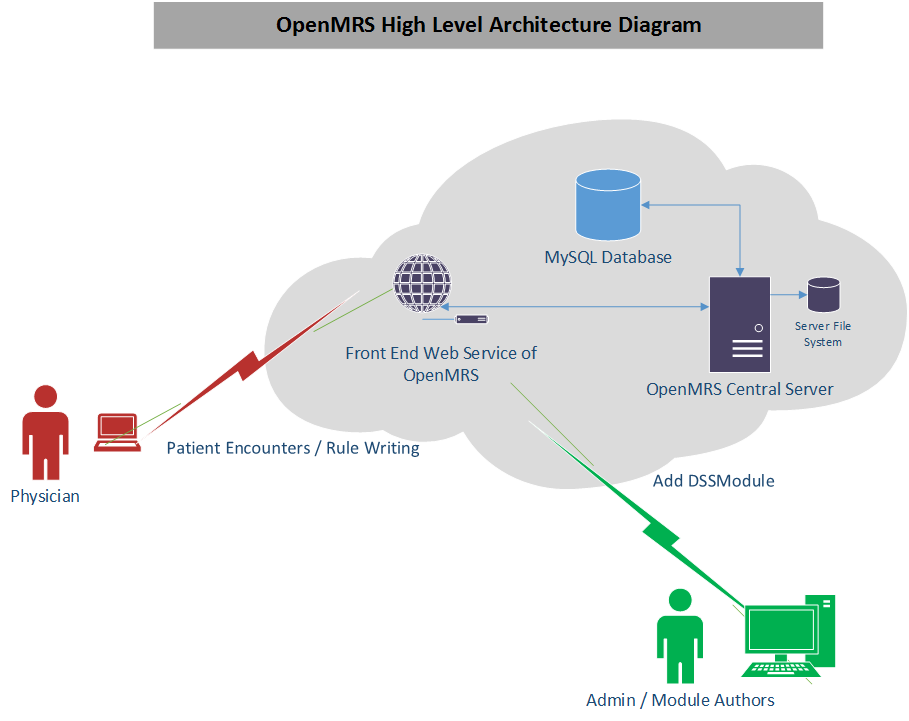
\includegraphics[width=6.5in]{OpenMRS_Architecture.png}
\end{center}
\caption{Architecture Diagram} \label{fig:ARCHITECTURE}
\end{figure}


\newpage 
\section{User guide}

\subsection{Rules}

A DSS rule is a program which examines patient data and, as 
appropriate, may issue alerts to specific pages within OpenMRS.

Links for manipulating DSS rules are found in the "DSS Compiler" 
section of the OpenMRS Administration page, as seen in Figure 
~\ref{fig:ADMINISTRATION}.

\begin{figure}\begin{center}
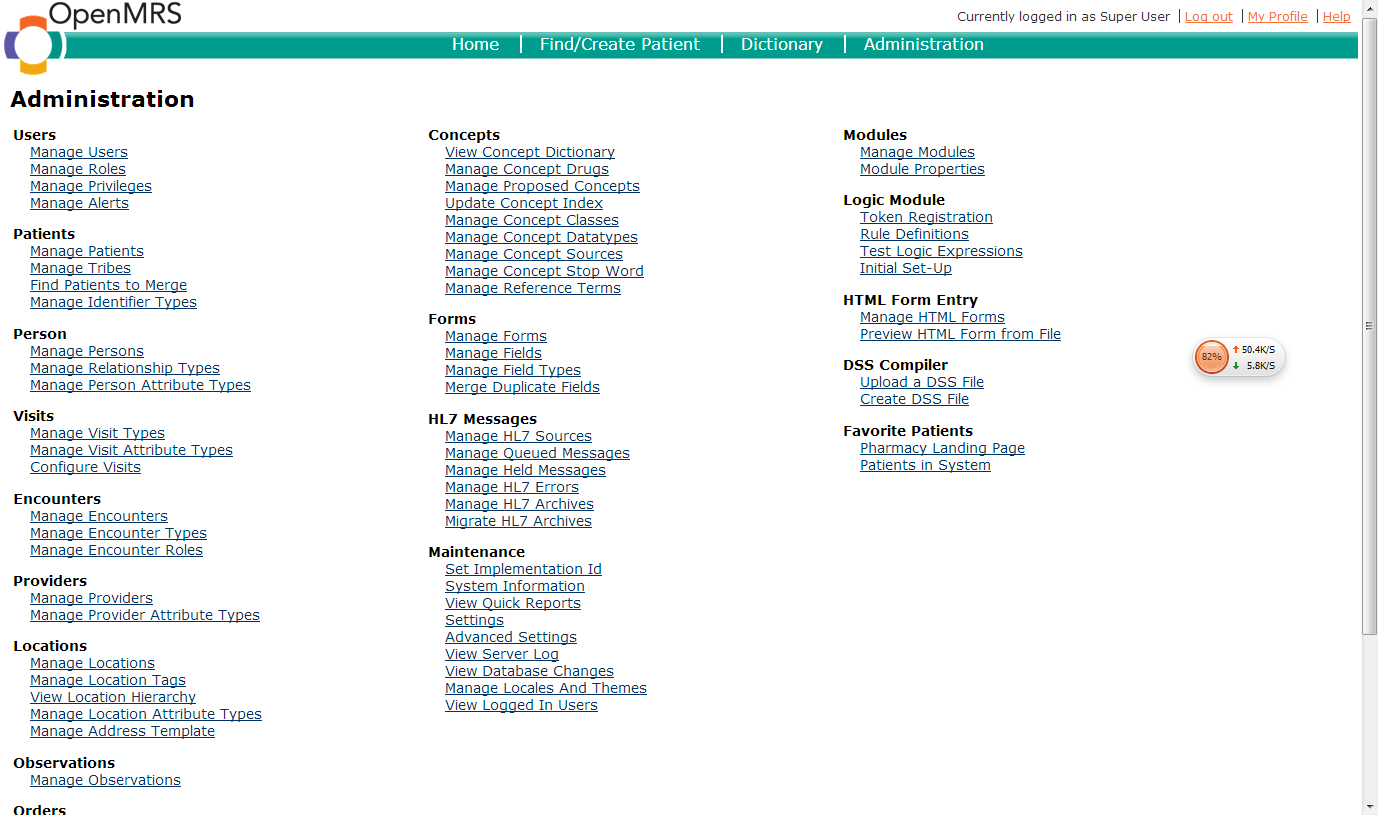
\includegraphics[width=6.5in]{administration.png}
\end{center}
\caption{OpenMRS Administration} \label{fig:ADMINISTRATION}
\end{figure}

\subsubsection{Creating a rule}

An OpenMRS user may create new rules using the "Create DSS Rule" 
link found on the Administration page. This page is shown in 
Figure ~\ref{fig:CREATE_DSS_PROGRAM}. The rule's author may 
enter a name and source code to the rule; pressing "Save" stores 
the rule to the DSS rule module.

\begin{figure}\begin{center}
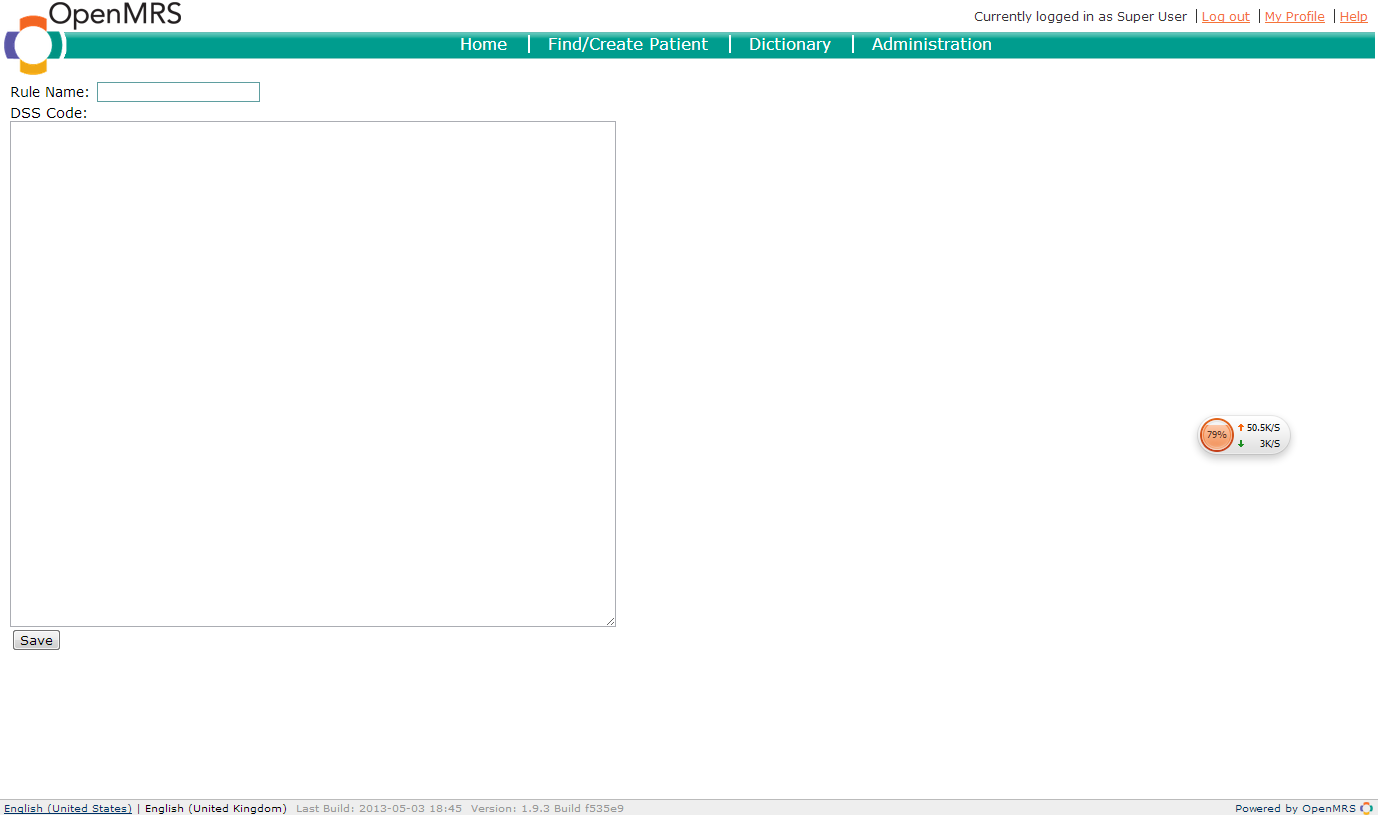
\includegraphics[width=6.5in]{createDSSProgram.png}
\end{center}
\caption{Creating a DSS Rule} \label{fig:CREATE_DSS_PROGRAM}
\end{figure}

\subsubsection{Modifying an existing rule}

\subsection{Alerts}

\subsubsection{Patient dashboard}

When viewing the Patient Dashboard, shown in Figure 
~\ref{fig:PATIENT_DASHBOARD_ALERT}, any relevant alerts for 
the patient appear in the top left. There is also a "View Summary" 
link to access the Patient Summary.

\begin{figure}\begin{center}
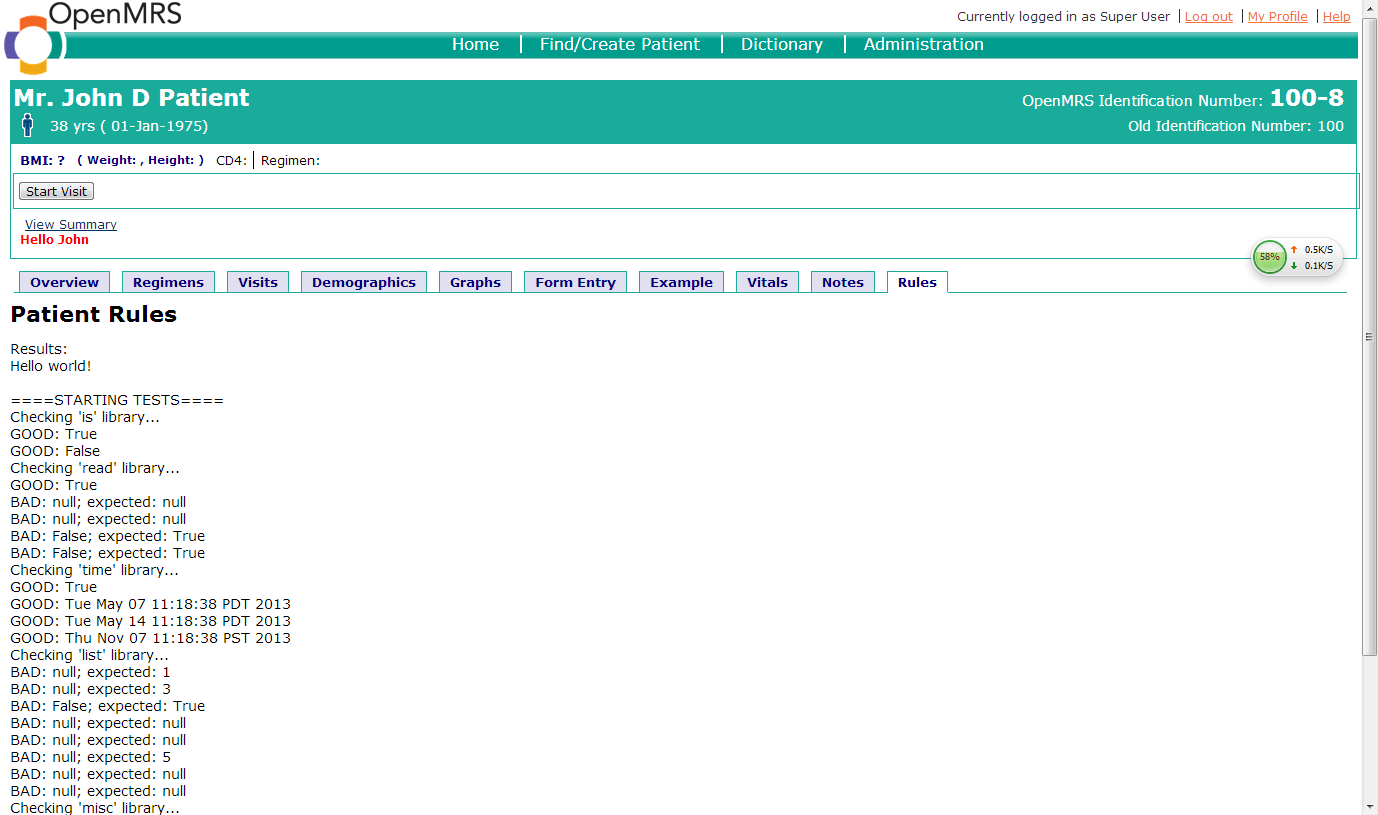
\includegraphics[width=6.5in]{dashboard2.png}
\end{center}
\caption{Patient Dashboard} \label{fig:PATIENT_DASHBOARD_ALERT}
\end{figure}

\subsubsection{Patient summary}

The Patient Summary, shown in Figure 
~\ref{fig:PATIENT_SUMMARY_ALERT}, shows certain relevant 
patient information, followed by any relevant alerts that are 
generated by the rule service.

\begin{figure}\begin{center}
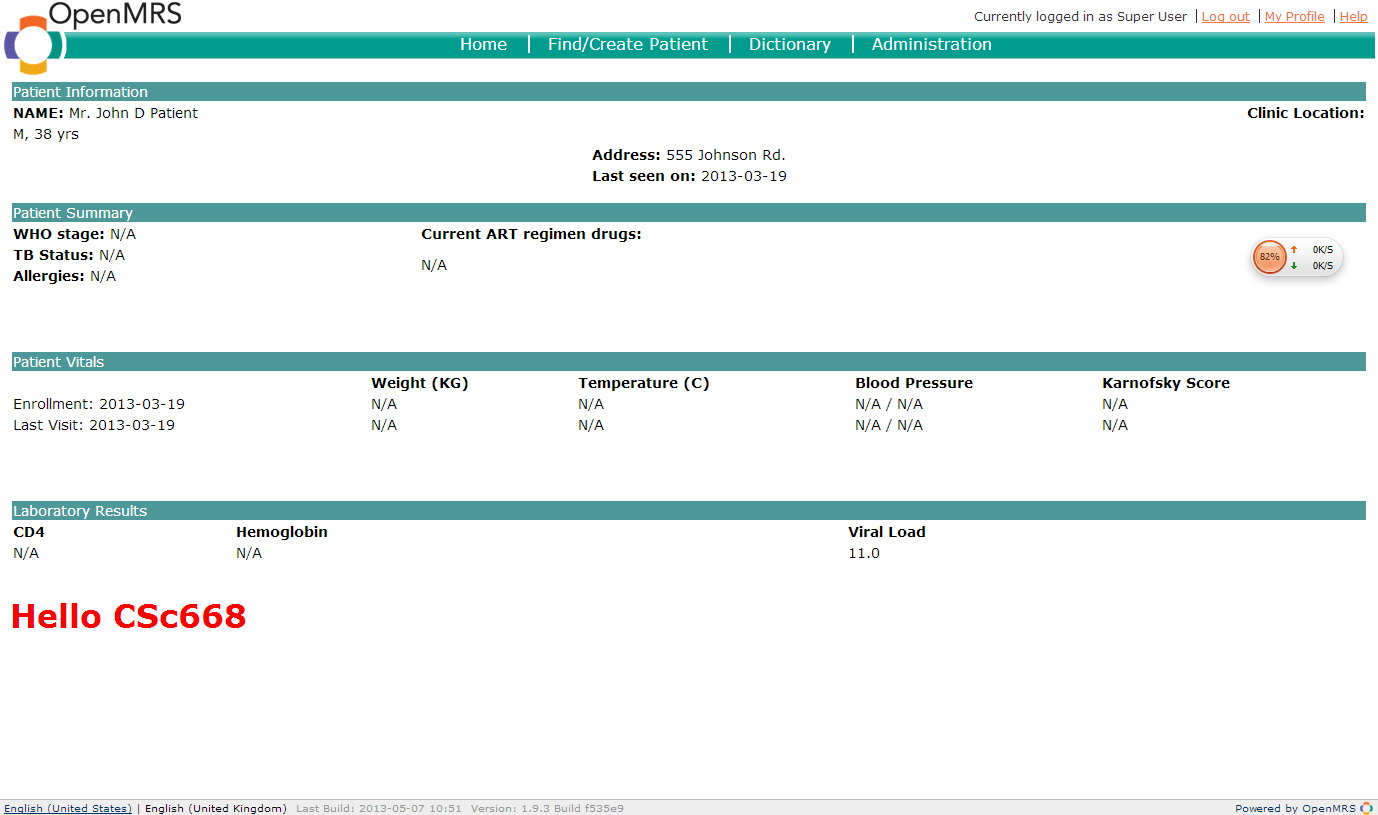
\includegraphics[width=6.5in]{summary.png}
\end{center}
\caption{Patient Summary} \label{fig:PATIENT_SUMMARY_ALERT}
\end{figure}

\newpage 
\section{Use cases}

\begin{figure}\begin{center}
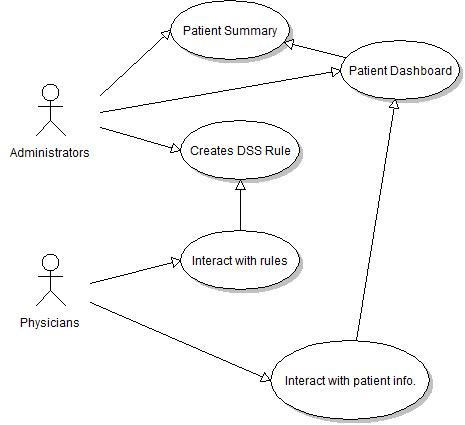
\includegraphics{use_case_diagram.png}
\end{center}
\caption{Use case overview}
\label{fig:USE_CASE_OVERVIEW}
\end{figure}

\subsection{Rule administration}

\subsection{Alerts}

\newpage 
\section{Sequence diagrams}

\begin{figure}\begin{center}
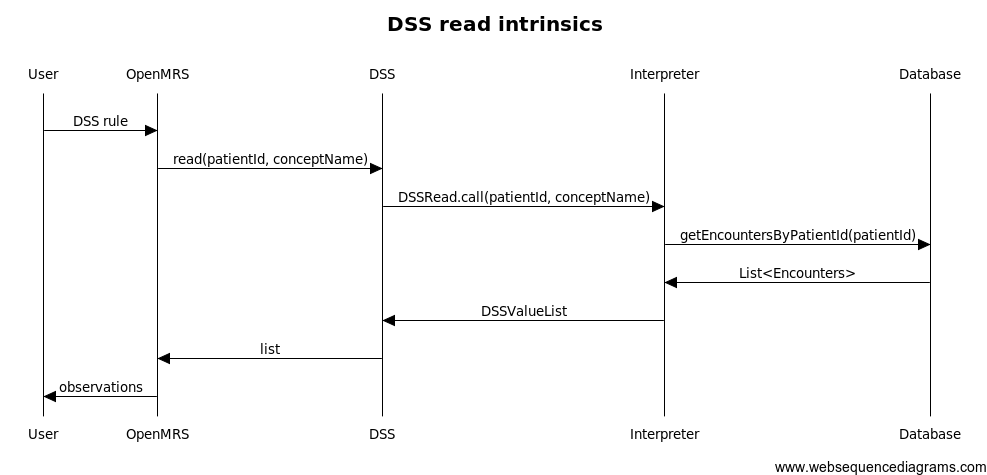
\includegraphics[width=6.5in]{readsequence.png}
\end{center}
\caption{Sequence diagram for read operation} 
\label{fig:SEQUENCE_READ}
\end{figure}


\newpage 
\section{Design overview} \label{sec:DESIGN_OVERVIEW}

	The DSS1 rule subsystem is incorporated into OpenMRS in a simple Client-Server fashion. The target implementation will feature client-side web pages which interact with the DSS1 rule subsystem on the server by way of DSSRuleService. Figure ~\ref{fig:TIERS} illustrates this interaction.

\tikzstyle{layer}=[rectangle, 
                   rounded corners,
                   draw=black, 
                   align=center,
                   anchor=north]
\tikzstyle{communicates}=[draw, ->, >=triangle 60]
\tikzstyle{boundary}=[draw, -, dashed]
\begin{figure}\begin{center}
\begin{tikzpicture}
\node (Client) [layer] { 
  \textbf{Client Pages}      \\
  Patient Summary \\
  Patient Dashboard \\
  DSS Rule Administration
};
\node (Boundary) [below=of Client, minimum width=3in] {};
\node [above=of Boundary.east] {\emph{Client}};
\node [below=of Boundary.east] {\emph{Server}};
\node (Service) [layer, below=of Boundary] { 
  \textbf{DSS Rule Service}  \\
  Run rules  \\
  List rules \\
  Add rules  \\
  Edit rules
};
\node (Interpreter) [layer, below=of Service] { 
  \textbf{DSS1 Interpreter}  \\
  Intrinsics  \\
  Evaluations \\
  Flow control
};
\path [communicates] (Client) -- (Service) {};
%\path [communicates] (Service.115    ) -- (Client.240     ) {};
\path [communicates] (Service) -- (Interpreter) {};
%\path [communicates] (Interpreter.120) -- (Service.245    ) {};
\path [boundary] (Boundary.180) -- (Boundary.0    ) {};
%\path [boundary]     (Boundary.west  ) -- (Boundary.east  ) {};
\end{tikzpicture}
\caption{Usage relationship of major tiers.}\label{fig:TIERS}
\end{center}\end{figure}

The DSS Rule Service, in turn, utilizing the DSS1 Interpreter subsystem to run rules and report results.

While the DSS Rule Service runs on the server, its interface is exposed to client-side JavaScript code via DWR (Direct Web Remoting).

\subsection{Client pages} \label{sec:CLIENT_PAGES}

Multiple client web pages interact with the DSS Rule Service.

\subsubsection{Patient summary} \label{sec:PATIENT_SUMMARY}

The Patient Summary ({\texttt{patientsummary.jsp}) is  stand-alone page, reachable from a link on the Patient Dashboard. It is used primarily to contain major information about a patient (gender, age, WHO stage, etc.) The Patient Summary invokes the rule service via DWR to retrieve all alerts for the named target  \texttt{summary} and displays them below other patient information. 

\subsubsection{Patient Dashboard} \label{sec:PATIENT_DASHBOARD}

The Patient Dashboard is the primary landing point for viewing patient information, and contains multiple tabs for this purpose. This extension inserts a link to the Patient Summary on the Patient Dashboard, and accompanies this with relevant alerts by invoking the rule service for the \texttt{dashboard} target.

See \texttt{org.openmrs.module.basicmodule.extension.html.PatientSummaryExtension}

\subsubsection {DSS Rule Administration} 
\label{sec:DSS_RULE_ADMINISTRATION}

Create DSS Rule (\texttt{dssRules.form}) provides a form where DSS source code can be entered and submitted to the rule service with a specific rule name. Consolidates the ability to create new rules, load existing rules, and edit rules in one form. Made accessible through an extension to the Administration menu.

\subsection{Rule service} \label{sec:RULE_SERVICE}

The DSSRuleService follows the facade design pattern to expose important functionality to clients. The high-level tasks that are relevant to client code are defined using a few simple methods which hide the details of compiling, interpreting, and managing the storage of rules. Specific functionality is detailed in table ~\ref{tab:RULE_SERVICE}.

\begin{table}
\begin{center}
\begin{tabular}{ l | p{1.25in} | p{2.25in} }
Method & Description & Details \\ \hline

\texttt{getRuleService()}
&
Static method to retrieve an instance of the rule service.
&
Constructs a new DSSRuleService object, if necessary. During 
constructor call any existing rules are loaded from the file 
system, using the XMLBuilder to convert from XML to DOM to AST.
\\ \hline

\texttt{store(rule, code)}
&
Stores a rule (either as a new rule, or replacing an existing rule) with the given source code.
&
Invokes the Parser to convert source code to AST; 
Invokes the XMLBuilder to convert AST to DOM and save; 
Saves the original source to file system for subsequent retrieval; 
Stores the AST in memory for subsequent running.
\\ \hline

\texttt{load(rule)}
&
Load the source code for an existing rule.
&
Reads stored source code from the file system.
\\ \hline

\texttt{listRules()}
&
List all existing rules.
&
Returns a list of all stored rule names.
\\ \hline

\texttt{runRules(patientId, target)}
&
Get all alerts for the given target (“summary” or “dashboard”) as appropriate to the given patient.
&
For each rule:
Construct interpreter; 
Install intrinsics, including “alert” function which stores to a map;
Pre-define “patientId” for DSS1 program;
Run the interpreter on the rule.
Thereafter, pull all alerts appropriate to the target from the map.
\\ \hline

\end{tabular}
\end{center}
\caption{Methods exposed by the DSS Rule Service}
\label{tab:RULE_SERVICE}
\end{table}

\subsubsection{Rule storage} \label{sec:RULE_STORAGE}

On upload, rules are compiled to an Abstract Syntax Tree (AST) form 
using the provided Parser class. Once compiled successfully, the rule is stored to the OpenMRS application data directory. 

Each rule is  stored in two formats: Plain text source code, and an XML (Extensible Markup Language) representation of the compiled AST. The 
source code is subsequently used only to support user interactions (for instance, if an administrator wants to load or modify source for an existing rule). The XML form is used when the DSS Rule Service is first initialized to load any existing rules from the file system. After initialization, rules are stored in memory as AST objects.

The utility class XMLBuilder is used for conversion between AST and XML. Internally, the class maintains a Document Object Model (DOM) representation of the AST. This can be either as loaded from an XML file, or as formed by traversing an AST. Likewise, XMLBuilder provides methods for both producing AST objects or writing XML files.

\subsection{Interpreter} \label{sec:INTERPRETER}

The Interpreter is implemented with four distinct sub systems, as depicted in Figure ~\ref{fig:INTERPRETER}.
At the top level, \emph{flow control} is provided by the InterpreterVisitor, which is responsible for traversing the Abstract Syntax Tree. An \emph{execution context} is maintained to describe the running state of the system, including defined variables and functions. While tree traversal coordinates complex expressions, the actual \emph{evaluation} of expressions is itself implemented in a distinct set of classes representing the types available under DSS1. Finally, a library of \emph{intrinsic functions} is provided in order to mediate interactions with OpenMRS from running DSS1, as well as to provide certain convenience functions to DSS1 rule programmers.

\tikzstyle{system}=[rectangle,
                   thick, 
                   draw=black, 
                   align=center,
                   anchor=north]
\tikzstyle{connects}=[draw, ->, >=triangle 60]
\tikzstyle{observes}=[draw, ->, dashed, >=triangle 60]
\begin{figure}
\begin{center}
\begin{tikzpicture}[node distance=1.5in]
\node (FlowControl) [system] 
      {\textbf{Flow control}};
\node (Middle) [below=of FlowControl] {};
\node (ExecutionContext) [system, left=of Middle] 
      {\textbf{Execution context}};
\node (Evaluation) [system, below=of Middle] 
      {\textbf{Evaluation}};
\node (IntrinsicFunction) [system, right=of Middle] 
      {\textbf{Intrinsic functions}};
\draw [connects] (FlowControl) -- (ExecutionContext) {}
      node [midway,above,sloped] {Sets, gets state} ;
\draw [connects] (ExecutionContext) -- (Evaluation) {}
      node [midway,below,sloped] {Contains values} ;
\draw [connects] (ExecutionContext) -- (IntrinsicFunction) {}
      node [midway,below left,sloped] {Contains functions} ;
\draw [connects] (FlowControl) -- (IntrinsicFunction) {}
      node [midway,above,sloped] {Invokes} ;
\draw [connects] (IntrinsicFunction) -- (Evaluation) {}
      node [midway,below,sloped] {Yields values} ;
\draw [connects] (FlowControl) -- (Evaluation) {}
      node [midway,above,sloped] {Assembles complex expressions} ;
\end{tikzpicture}
\end{center}
\caption{High-level overview of the DSS1 Interpreter.}
\label{fig:INTERPRETER}
\end{figure}

\subsubsection{Flow control} \label{sec:FLOW_CONTROL}

	Flow control in the interpreter is implemented using the Visitor design pattern, traversing the Abstract Syntax Tree (AST) produced by the existing Compiler using an implementation of the provided ASTVisitor interface, performing computation as appropriate at every given node in the tree.

	The Visitor design pattern leverages double dispatch to decouple a data structure from the operations which can be performed while traversing this data structure. The Visitor calls an \texttt{accept} method on a node within the data structure, which is itself overloaded to call a more specific method on the Visitor itself; \texttt{visitBlockTree}, for example. This permits the external object – the Visitor – to implement behavior using the data structure's type hierarchy, without adding that specific behavior to those types directly.

	In the case of the Interpreter, the data structure is the AST, which describes a DSS1 program as a tree of elements – block (BlockTree), if statements (IfTree), et cetera. The Visitor is the IntepreterVisitor, which manages and performs the computation described by this program. This is done with the support of other underlying subsystems to describe variable state and perform type-specific evaluations, as described in the Architecture section.

	The class InterpreterVisitor acts as the center of a subsystem  responsible for high-level interpretation of the program, including flow control, and coordinating complex expressions.

\subsubsection{Execution context} \label{sec:EXECUTION_CONTEXT}

The ExecutionContext class provides a means to store and retrieve return values, variable states, and named functions. It also handles rules of scope to hide variables during function calls, and exposes the Evaluator. Note that this may be populated with functions or even variables before being given to the InterpreterVisitor, allowing the definition of intrinsics and constants (such as \texttt{patientId}).

Functions stored in the ExecutionContext are of type DSSFunction, which is an interface used to describe any function called from DSS1 (either intrinsic or user-defined). This permits function calling to be implemented identically for both categories of function. Additionally includes a method for testing if a given argument should be passed as a raw identifier instead of evaluated directly (as used by some intrinsics.).

Similarly, variables and return values are stored as DSSValue 
objects, with their specific implementation defined within the 
evaluation subsystem.

\subsubsection{Evaluation of expressions} \label{sec:EVALUATION}

The abstract class DSSValue describes a set of operations which can be performed on values in DSS1 as methods, as well as the common state (the potential to store time stamps). Its concrete sub-classes, such as DSSValueInt, DSSValueFloat, et cetera, provide specific implementations of these operations in order to define the behavior of their DSS1 type. Additionally, concrete subclasses of DSSValue typically are defined with some field to maintain their specific value (for instance, DSSValueBool has an underlying Java \texttt{boolean} field to describe its value.)

The Evaluator interface and DSSEvaluator implementation exposes methods to perform operations upon DSS1 values, to interpret literals, allocate DSS objects, and perform conversions between DSS1 values and similar Java objects. The Evaluator serves as intermediary between flow control and the specific semantics implemented in DSSValue types; this facilitates separation of concerns, allowing the gradual introduction of new DSS1 data types while avoiding changes to  flow control.

Finally, a DSSValueFactory class is provided to aid in the instantiation of DSSValue objects. This class utilizes the Factory design pattern to allow new values to be created (for instance, as the return values of intrinsic functions) without requiring users of those values to have specific knowledge of the DSSValue subclasses actually used.

\subsubsection{Intrinsic functions} \label{sec:INTRINSIC_FUNCTIONS}

DSSLibrary defines an interface for delivering or generating intrinsic functions in related groupings. Each function is returned in a map where the name should be used to call the function from a DSS program, and the function object is used as a Java object that extends the DSSFunction. These functions may then be easily installed into the ExecutionContext used by the Intepreter before running rules. A list of libraries used in this implementation is presented in Table ~\ref{tab:LIBRARIES}.

This approach supports extensibility of the DSS rule module. 
Rather than being built into the DSS1 Interpreter at the language 
level, intrinsic functions can be contained and communicated 
as DSSLibrary objects. Adding intrinsics is then as simple as 
defining a new DSSLibrary and installing it to the execution context before running rules.

The ReadLibrary serves as an interesting example case, at it illustrates interaction with the OpenMRS platform without requiring specific knowledge of this platform from other elements of the interpreter. The read functions retrieve a list of observations associated with a patient. The first parameter of the functions, patientId, is a numeric identifier unique to each patient. The second parameter, conceptName, is the word or phrase used by the OpenMRS dictionary to refer to a concept. 

The three functions are nearly identical, save for one difference: while read() returns a list containing all observations that match the function parameters, readInitialEncounter() and readLatestEncounter() filter out results based on the timestamp of the observations. Calling readInitialEncounter() retrieves only the observations from the patient's earliest encounter on record, while readLatestEncounter() retrieves only the observations from the patient's most recent encounter on record. 

When the functions are called, they retrieve a list of all encounters associated with patientId from the OpenMRS database. The functions iterate through these lists, and in the case of readInitialEncounter() and readLatestEncounter(), the timestamp for each encounter is checked. If the timestamp does not meet the criteria, the encounter is discarded. Once an encounter has been verified as valid the function shall retrieve all observations associated with the encounter. Each observation shall have its concept name checked against conceptName, and matches are added to the list of observations that each function shall return. 

Observations consist of three pieces of data: the value of the observation, the data type of the observation value, and the time of the observation. Internally, observations are represented as DSSValue objects, which store the value of the observation and the time of the observation. The data type of the observation value is stored as part of the DSSValue class type itself. Both the time and data type of the observation can be retrieved using the time() and type check intrinsics, respectively. 

Note that the \texttt{alert} intrinsic is treated as a special case. Rather than being contained within a library class, it is installed directly by the DSS Rule Service into the Interpreter before running rules. This facilitates retrieval of results issued via \texttt{alert} calls.

\begin{table}
\begin{center}
\begin{tabular} { l | l }
\textbf{Library}  & \textbf{Functions implemented}\\ \hline
IsLibrary         & \texttt{isString(var)}        \\
                  & \texttt{isFloat(var)}         \\
                  & \texttt{isInt(var)}           \\
                  & \texttt{isBoolean(var)}       \\
                  & \texttt{isList(var)}          \\
                  & \texttt{isObject(var)}        \\
                  & \texttt{isDate(var)}          \\ \hline
LengthAndWithinLibrary
                  & \texttt{length(var)}          \\
                  & \texttt{within(v,a,b)}        \\ \hline
ListLibrary       & \texttt{merge(a,b)}           \\
                  & \texttt{sortTime(list)}       \\
                  & \texttt{sortData(list)}       \\
                  & \texttt{first(list)}          \\
                  & \texttt{last(list)}           \\ \hline
ReadLibrary       & \texttt{read(patientId,
                                 concept)}        \\
                  & \texttt{readInitialEncounter(patientId,
                                 concept)}        \\
                  & \texttt{readLatestEncounter(patientId,
                                 concept)}        \\ \hline
DateLibrary       & \texttt{currenttime()}        \\
                  & \texttt{recentTimeItem(list)} \\
                  & \texttt{oldestTimeItem(list)} \\
                  & \texttt{before(a,b)}          \\
                  & \texttt{time(var)}            \\
                  & \texttt{addDays(v,days)}      \\
                  & \texttt{addMonths(v,months)}  \\ \hline
\end{tabular}
\end{center}
\caption{Libraries of intrinsics}
\label{tab:LIBRARIES}
\end{table}

% \section{External documentation}

\newpage 
\section{Package diagrams}

\newpage 
\section{Class diagrams} \label{sec:CLASS_DIAGRAMS}

\subsection{Classes describing flow control}

Figure ~\ref{fig:INTERPRETER_VISITOR_DIAGRAM} shows the relationship 
of classes directly involved in or utilized during the handling of flow 
control when interpreting a DSS program.

The InterpreterVisitor is used to initiate program interpretation. It 
delegates the interpretation of specific node types to corresponding 
ASTInterpreter types. It also maintains an instance of a DSSExecutionContext 
to support interactions with the running state of the program.

\subsection{Classes describing execution context}

Figure ~\ref{fig:EXECUTION_CONTEXT_DIAGRAM} describes the 
composition of the execution context. The active state of the program, 
including currently-defined functions and variable assignments, is maintained in appropriate data structures.

Each ExecutionContext additionally maintains a reference to an Evaluator 
object, which exposes necessary methods for the interpreter to interact 
with values in DSS.

\subsection{Classes describing values}

Figure ~\ref{fig:VALUE_DIAGRAM} shows the classes used to describe values in 
a running DSS program. The abstract class DSSValue describes the operations 
available under DSS1 as methods; its concrete subclasses provide 
implementations for these operations. Note that each DSSValue object also 
maintains a field for the time stamp of a value, which is populated when 
observations are read from OpenMRS services. For other values this is null.

Not shown is DSSValueFactory, which exposes methods to create DSSValue 
objects to wrap their corresponding underlying Java types.

\subsection{Classes describing intrinsics}

Figure ~\ref{fig:INTRINSIC_DIAGRAM} describes the relationship of classes 
which describe specific intrinsic functions to the classes used to 
categorize them.

Calls made by a running DSS program are resolved by a named DSSFunction 
object, as stored in the execution context. The DSSLibrary interface 
provides a useful way to group related functions along with their names 
to facilitate their installation into the execution context. 

Also shown is the DeclaredFunction class. A DeclaredFunction is created 
for user-defined functions in a DSS program, and contains references to 
appropriate nodes within the AST to support actual interpretation of the 
function call, as well as the visitor used to perform interpretation, and 
the execution context, which is used to handle the change in variable 
scope associated with the function call.

\tikzstyle{class}=[rectangle, 
                   draw=black, 
                   rectangle split, 
                   rectangle split parts=3,
                   align=center,
                   anchor=north]
\tikzstyle{implements}=[draw, ->, >=open triangle 90]
\tikzstyle{aggregates}=[draw, <-, >=open diamond]
\tikzstyle{contains}=[draw, <-, >=diamond]

\begin{figure}
\begin{center}
\begin{tikzpicture}[node distance=0.25in]
\node (ASTVisitor) [class] { 
  \emph{ASTVisitor}
  \nodepart{second}  
  \nodepart[align=justify]{third}
  + visitBlockTree(t : AST) \\
  + visitIdTree(t : AST)    \\
  + visitCallTree(t : AST)  \\
  ...
};
\node (InterpreterVisitor) [class, below=of ASTVisitor] { 
  \textbf{InterpreterVisitor}
  \nodepart{second}  
  \nodepart[align=justify]{third}
};

\node (DSSExecutionContext) [class, right=of InterpreterVisitor] { 
  \textbf{DSSExecutionContext}
  \nodepart{second}  
  \nodepart[align=justify]{third}
  + setConstant(name : String,  value : DSSValue) \\
  + setIntrinsic(name : String,  func : DSSFunction)
};
\node (ExecutionContext) [class, above=of DSSExecutionContext] { 
  \textbf{ExecutionContext}
  \nodepart[align=justify]{second}  
  - evaluator : Evaluator
  \nodepart[align=justify]{third}
  + beginScope() \\
  + endScope() \\
  + getEvaluator() : Evaluator \\
  + getFunction(name : String) : DSSFunction \\
  + getReturnValue() : DSSValue \\
  + setReturnValue(v : DSSValue) \\
  + setFunction(name : String, f : DSSFunction)
};
\node (ASTInterpreter) [class, below=of InterpreterVisitor.south east] { 
  \emph{ASTInterpreter}
  \nodepart{second}  
  \nodepart[align=justify]{third}
  + interpret(ast : AST, 
              c : ExecutionContext, 
              v : ASTVisitor) \\ \hspace{10pt} : Object
};

\node (IdInterpreter) [class, below=of ASTInterpreter] { 
  \textbf{IdInterpreter}
  \nodepart{second}  
  \nodepart[align=justify]{third}
};
\node (BlockInterpreter) [class, left=of IdInterpreter] { 
  \textbf{BlockInterpreter}
  \nodepart{second}  
  \nodepart[align=justify]{third}
};
\node (CallInterpreter) [class, right=of IdInterpreter] { 
  \textbf{CallInterpreter}
  \nodepart{second}  
  \nodepart[align=justify]{third}
};
\node () [right=of CallInterpreter] {...};


\node (NamingContext) [class, above=of ExecutionContext] { 
  \emph{NamingContext}
  \nodepart[align=justify]{third}
  +set (name : String, value : DSSValue) \\
  +get (name : String) : DSSValue
};

\path [implements] (ExecutionContext) -- (NamingContext) {};
\path [implements] (InterpreterVisitor) -- (ASTVisitor) {};
\path [implements] (BlockInterpreter) -- (ASTInterpreter) {};
\path [implements] (IdInterpreter) -- (ASTInterpreter) {};
\path [implements] (CallInterpreter) -- (ASTInterpreter) {};
\path [implements] (DSSExecutionContext) -- (ExecutionContext) {};
\path [contains] (InterpreterVisitor) -- (DSSExecutionContext) {};
\path [contains] (InterpreterVisitor) -- (ASTInterpreter) {};
\draw (InterpreterVisitor) -- (ASTInterpreter) 
      node [midway, right] {\small{1..*}};
\draw (InterpreterVisitor) -- (DSSExecutionContext) 
      node [midway, above] {\small{1..1}};
\end{tikzpicture}
\end{center}
\caption{Interpreter visitor}
\label{fig:INTERPRETER_VISITOR_DIAGRAM}
\end{figure}

\begin{figure}
\begin{tikzpicture}[node distance=0.33in]
\node (ExecutionContext) [class] { 
  \textbf{ExecutionContext}
  \nodepart[align=justify]{second}  
  - functions : Map\textless String, DSSFunction\textgreater \\
  - variables : Map\textless String, DSSValue\textgreater \\
  - scope : Stack\textless Map\textless String, DSSValue\textgreater \textgreater \\
  - returnValue : DSSValue \\
  - evaluator : Evaluator
  \nodepart[align=justify]{third}
  + beginScope() \\
  + endScope() \\
  + getEvaluator() : Evaluator \\
  + getFunction(name : String) : DSSFunction \\
  + getReturnValue() : DSSValue \\
  + setReturnValue(v : DSSValue) \\
  + setFunction(name : String, f : DSSFunction)
};
\node (DSSValue) [class, right=of ExecutionContext] { 
  \emph{DSSValue}
  \nodepart[align=justify]{second}  
  - timestamp : Date
  \nodepart[align=justify]{third}
  + add (v : DSSValue) : DSSValue \\
  + sub (v : DSSValue) : DSSValue \\
  + div (v : DSSValue) : DSSValue \\
  ... \\
  + getTimeStamp() : Date
};
\node (NamingContext) [class, above=of ExecutionContext] { 
  \emph{NamingContext}
  \nodepart[align=justify]{third}
  +set (name : String, value : DSSValue) \\
  +get (name : String) : DSSValue
};
\node (DSSFunction) [class, right=of NamingContext] { 
  \emph{DSSFunction}
  \nodepart{second}  
  \nodepart[align=justify]{third}
  + call(args : DSSValue[]) : DSSValue \\
  + passAsIdentifier(argIndex : int) \\ \hspace{10pt} : boolean
};

\node (Evaluator) [class, below=of ExecutionContext] { 
  \emph{Evaluator}
  \nodepart{second}  
  \nodepart[align=justify]{third}
  + castTo(javaClass : Class, v : DSSValue) : Object \\
  + evaluate(leftOper : DSSValue, \\ 
    \hspace{10pt} operator : String, \\
    \hspace{10pt} rightOper : DSSValue) : DSSValue\\
  + evaluateLiteral(lit : Symbol) : DSSValue \\
  + newAllocation(fields : String[]) : DSSValue \\
  + toDSSValue(javaObject : Object) : DSSValue
};
\node (DSSEvaluator) [class, right=of Evaluator] { 
  \textbf{DSSEvaluator}
  \nodepart{second}  
  \nodepart[align=justify]{third}
};


\path [aggregates] (ExecutionContext) -- (DSSValue) {};
\path [aggregates] (ExecutionContext) -- (DSSFunction) {};
\path [contains] (ExecutionContext) -- (Evaluator) {};
\path [implements] (ExecutionContext) -- (NamingContext) {};
\path [implements] (DSSEvaluator) -- (Evaluator) {};
\draw (ExecutionContext) -- (DSSValue) 
      node [midway, above] {\small{1..*}};
\draw (ExecutionContext) -- (DSSFunction) 
      node [midway, below] {\small{1..*}};

\end{tikzpicture}
\caption{Execution context class diagram}
\label{fig:EXECUTION_CONTEXT_DIAGRAM}
\end{figure}

\begin{figure}
\begin{center}
\begin{tikzpicture}[node distance=0.25in]
\node (DSSValue) [class] { 
  \emph{DSSValue}
  \nodepart[align=justify]{second}  
  - timestamp : Date
  \nodepart[align=justify]{third}
  + add (v : DSSValue) : DSSValue \\
  + sub (v : DSSValue) : DSSValue \\
  + div (v : DSSValue) : DSSValue \\
  + mul (v : DSSValue) : DSSValue \\
  + power (v : DSSValue) : DSSValue \\
  + concat (v : DSSValue) : DSSValue \\
  + and (v : DSSValue) : DSSValue \\
  + or (v : DSSValue) : DSSValue \\
  + equal (v : DSSValue) : boolean \\
  + notequal (v : DSSValue) : boolean \\
  + lessthan (v : DSSValue) : boolean \\
  + greaterthan (v : DSSValue) : boolean \\
  + lessthanequal (v : DSSValue) : boolean \\
  + greaterthanequal (v : DSSValue) : boolean \\
  + getTimeStamp() : Date \\
  + setTimeStamp(date : Date)
};

\node (DSSValueNumeric) [class, right=of DSSValue.north east] {
  \emph{DSSValueNumeric}
  \nodepart[align=justify]{second}  
  \nodepart[align=justify]{third}
};
\node (DSSValueFloat) [class, above=of DSSValueNumeric] {
  \textbf{DSSValueFloat}
  \nodepart[align=justify]{second}  
  - value : double
  \nodepart[align=justify]{third}
};
\node (DSSValueInt) [class, below=of DSSValueNumeric] {
  \textbf{DSSValueInt}
  \nodepart[align=justify]{second}  
  - value : long
  \nodepart[align=justify]{third}
};
\node (DSSValueBool) [class, below=of DSSValueInt] {
  \textbf{DSSValueBool}
  \nodepart[align=justify]{second}  
  - value : boolean
  \nodepart[align=justify]{third}
};
\node (DSSValueString) [class, below=of DSSValueBool] {
  \textbf{DSSValueString}
  \nodepart[align=justify]{second}  
  - value : String
  \nodepart[align=justify]{third}
};
\node (DSSValueList) [class, below=of DSSValueString] {
  \textbf{DSSValueList}
  \nodepart[align=justify]{second}  
  - value : List
  \nodepart[align=justify]{third}
};
\node (DSSValueObject) [class, below=of DSSValue] {
  \textbf{DSSValueObject}
  \nodepart[align=justify]{second}  
  - fields : Map\textless String, DSSValue\textgreater 
  \nodepart[align=justify]{third}
};
\node (DSSValueNull) [class, right=of DSSValueObject] {
  \textbf{DSSValueNull}
  \nodepart[align=justify]{second}  
  \nodepart[align=justify]{third}
};

\node (NamingContext) [class, below=of DSSValueObject] { 
  \emph{NamingContext}
  \nodepart[align=justify]{third}
  +set (name : String, value : DSSValue) \\
  +get (name : String) : DSSValue
};

\path [implements] (DSSValueInt) -- (DSSValueNumeric) {};
\path [implements] (DSSValueFloat) -- (DSSValueNumeric) {};
\path [implements] (DSSValueNumeric) -- (DSSValue) {};
\path [implements] (DSSValueBool) -- (DSSValue) {};
\path [implements] (DSSValueString) -- (DSSValue) {};
\path [implements] (DSSValueList) -- (DSSValue) {};
\path [implements] (DSSValueNull) -- (DSSValue) {};
\path [implements] (DSSValueObject) -- (DSSValue) {};
\path [implements] (DSSValueObject) -- (NamingContext) {};
\end{tikzpicture}
\end{center}
\caption{Value class diagram}
\label{fig:VALUE_DIAGRAM}
\end{figure}

\begin{figure}
\begin{center}
\begin{tikzpicture}[node distance=0.25in]
\node (DSSLibrary) [class] { 
  \emph{DSSLibrary}
  \nodepart[align=justify]{second}  
  \nodepart[align=justify]{third}
  +getFunctions(context : ExecutionContext) : 
      Map \textless String, DSSFunction\textgreater
};

\node (ReadLibrary) [class, below=of DSSLibrary] { 
  \textbf{ReadLibrary}
  \nodepart[align=justify]{second}  
  \nodepart[align=justify]{third}
};

\node (DateLibrary) [class, left=of ReadLibrary] { 
  \textbf{DateLibrary}
  \nodepart[align=justify]{second}  
  \nodepart[align=justify]{third}
};

\node (ListLibrary) [class, right=of ReadLibrary] { 
  \textbf{ListLibrary}
  \nodepart[align=justify]{second}  
  \nodepart[align=justify]{third}
};

\node (DSSRead) [class, below=of ReadLibrary] { 
  \textbf{DSSRead}
  \nodepart[align=justify]{second}  
  \nodepart[align=justify]{third}
};

\node (DSSReadInitialEncounter) [class, left=of DSSRead] { 
  \textbf{DSSReadInitialEncounter}
  \nodepart[align=justify]{second}  
  \nodepart[align=justify]{third}
};

\node (DSSReadLatestEncounter) [class, right=of DSSRead] { 
  \textbf{DSSReadLatestEncounter}
  \nodepart[align=justify]{second}  
  \nodepart[align=justify]{third}
};

\node (DSSFunction) [class, below=of DSSRead] { 
  \emph{DSSFunction}
  \nodepart{second}  
  \nodepart[align=justify]{third}
  + call(args : DSSValue[]) : DSSValue \\
  + passAsIdentifier(argIndex : int)  : boolean
};

\node (DeclaredFunction) [class, below=of DSSFunction] { 
  \textbf{DeclaredFunction}
  \nodepart[align=justify]{second}  
  formals : FormalsTree \\
  block : BlockTree \\
  context : ExecutionContext \\
  visitor : ASTVisitor
  \nodepart[align=justify]{third}
};

\node () [left=of DateLibrary] {...};
\node () [right=of ListLibrary] {...};
\node () [left=of DSSReadInitialEncounter] {...};
\node () [right=of DSSReadLatestEncounter] {...};


\path [contains] (ReadLibrary) -- (DSSRead) {};
\path [contains] (ReadLibrary) -- (DSSReadInitialEncounter) {};
\path [contains] (ReadLibrary) -- (DSSReadLatestEncounter) {};
\path [implements] (ReadLibrary) -- (DSSLibrary) {};
\path [implements] (DateLibrary) -- (DSSLibrary) {};
\path [implements] (ListLibrary) -- (DSSLibrary) {};
\path [implements] (DSSRead) -- (DSSFunction) {};
\path [implements] (DSSReadInitialEncounter) -- (DSSFunction) {};
\path [implements] (DSSReadLatestEncounter) -- (DSSFunction) {};
\path [implements] (DeclaredFunction) -- (DSSFunction) {};


\end{tikzpicture}
\end{center}
\caption{Intrinsic class diagram}
\label{fig:INTRINSIC_DIAGRAM}
\end{figure}

\newpage \appendix 
\section{DSS1 Grammar}
\begin{verbatim}
 PROGRAM -> ‘program’ D* BLOCK ==> program
 BLOCK -> ‘{‘ S* ‘}’  ==> block
 D -> 'function' NAME FUNHEAD BLOCK      	==> functionDecl
 FUNHEAD  -> '(' (NAME list ',')? ')'  	==> formals
 S -> ‘if’ EE ‘then’ BLOCK ('else' BLOCK)? ==> if 
   -> ‘if’ EE ‘then’ BLOCK Elif ==> if 
   -> ‘while’ EE BLOCK               		==> while
   -> 'for' NAME in NLIST BLOCK     		==> FOR
   -> ‘return’ EE                    		==> return
   -> BLOCK
   -> IdMod’:=‘ EE                    		==> assign
   -> NAME '(' (EE list ',')? ')' 		==> call
 
  Elif -> ‘elsif’ EE 'then' BLOCK Elif			==> elsif
-> ‘elsif’ EE 'then' BLOCK ('else' BLOCK)?	==> elsif
  
  EE 	-> E
  	-> EE '||' E
  
  E 	-> SE
  	-> SE ‘==‘ SE   	==> =
  	-> SE ‘!=‘ SE   	==> !=
  	-> SE ‘<‘  SE   	==> <
  	-> SE ‘<=‘ SE   	==> <=
 
  SE 	->  T
  	->  SE ‘+’ T  	==> +
  	->  SE ‘-’ T  	==> -
  	->  SE ‘|’ T  	==> or
 
  T  	-> TT
  	-> T ‘*‘ F  	==> *
  	-> T ‘/’ F  	==> /
  	-> T ‘&’ F  	==> and
 
  TT 	-> F
  	-> TT ** F    	==> **
 
  F  	-> ‘(‘ EE ‘)’
  	-> IdMod 
  	-> <literal>
  	-> NAME '(' (EE list ',')? ')' 		==> call
  	-> Object '(' (NAME list ',')? ')'    ==> ObjectDecl
  	-> new NAME          				==> Object
  	-> LIST
  IdMod -> NAME
        -> NAME '.' NAME    			==> fieldRef
  
  NLIST	-> NAME
       	-> LIST
  
  LIST	-> '{' (E list ',')? '}'   		==> list
 
  NAME	-> <id>
\end{verbatim}

\newpage
\section{Test cases}

\newpage
\section{API Documentation}



\end{document}